\documentclass[12pt]{article}%
\usepackage{amsfonts}
\usepackage{fancyhdr}
\usepackage{comment}
\usepackage{mathrsfs}
\usepackage{graphicx}
\usepackage[a4paper, top=2.5cm, bottom=2.5cm, left=2.2cm, right=2.2cm]%
{geometry}
\usepackage{times}
\usepackage{amsmath}
%\usepackage{changepage}
\usepackage{amssymb}
\usepackage{amsthm}
\usepackage{float}
%\usepackage{graphicx}%

\newcommand{\Q}{\mathbb{Q}}
\newcommand{\R}{\mathbb{R}}
\newcommand{\C}{\mathbb{C}}
\newcommand{\Z}{\mathbb{Z}}

\newcommand{\E}{\mathrm{E}}
\newcommand{\Var}{\mathrm{Var}}
\newcommand{\Cov}{\mathrm{Cov}}

\begin{document}

\title{Math 545 - PDE - Homework 6}
\author{YingLi, Fernando, Laurette }
\date{\today}
\maketitle

\section*{Section 14.1}
\subsection*{Exercise 2} 
Solve $(1+t)u_{t}+xu_{x}=0$. Then solve it with the initial condition $u(x,0)=x^5$ for $t>0$.\\
\textbf{Solution:}\\
The characteristic equation is 
\begin{equation*}
    \begin{cases}
     \dot{X} =\frac{x}{1+t}, \\
      X(0,x) =x.
    \end{cases}
\end{equation*}
%This ODE seperates as $\frac{dx}{x}=\frac{dt}{1+t}$, integrating in the both sides, $X=C(1+t)$, and $X(0,x)=C=x$. 
Solve this ODE, the solution is $X(t,x)=x(1+t)$.\\
Fix $X$, along characteristic curve, transfer $X\to x, x\to x_{0}$, then $x=x_{0}(1+t)\implies x_{0}=\frac{x}{1+t} $.\\
%$X(t_{0}, y(t_{0},x_{0}))=x_{0}=y(1+t_{0})\implies y=\frac{x_{0}}{1+t_{0}}$.\\
%Thus , $u(t_{0},x_{0})=u_{0}(y(t_{0},x_{0}))=(\frac{x_{0}}{1+t_{0}})^5$.
Along the characteristic curve, $u(t,x)=u(0,x_{0})=(\frac{x}{1+t})^5$.\\
Therefore, the solution  is $u(t,x)=(\frac{x}{1+t})^5. $




\subsection*{Exercise 3}
Solve the nonlinear equation $u_{t}+uu_{x}=0$ with the auxiliary condition $u(x,0)=x$. Sketch some of the characteristic lines.\\
\textbf{Solution:}\\
The characteristic equation is \begin{equation*}
    \begin{cases}
     \dot{X} =u(x,t)=constant, \\
      X(0,x) =x.
    \end{cases}
\end{equation*} %Along characteristic curve, $u(x,t)$ is a constant.\\ %Thus each characteristic curve is a straight line. \\
%Consider the characteristic line passing through $(x_{0},0)$ and $(x,t)$. Its slope is 
%\[\frac{x-x_{0}}{t-t_{0}}=\frac{dx}{dt}=u(x,t)=u(x_{0},0)=\phi(x_{0})\implies x=t\phi(x_{0})+x_{0}.\]
%From the initial condition, $\phi(x_{0})=x_{0}$, so $x=x_{0}+tx_{0}$.\\
Fix $X$, along $X$, transfer $X\to x, x\to x_{0}$, then $x=tu(x_{0},0)+x_{0}\implies x_{0}=\frac{x}{1+t}$.\\
The solution is $u(x,t)=u(x_{0},0)=x_{0}=\frac{x}{1+t}.$\\
Sketch some of the characteristic lines:

\begin{figure}[h]
    \centering
    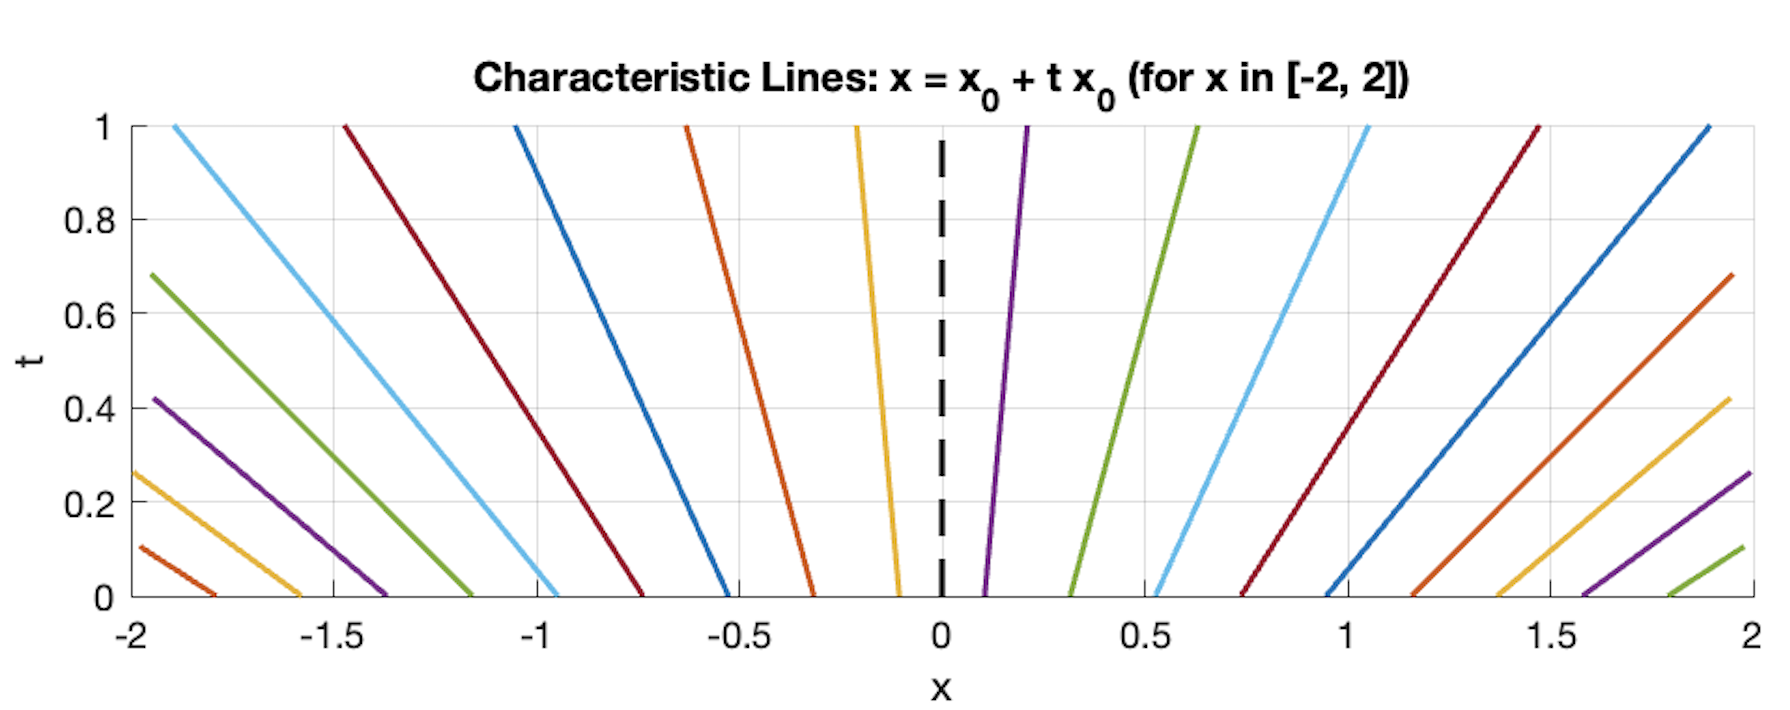
\includegraphics[width=0.65\textwidth]{Graph 1.png} % Replace "filename" with the actual name of your image file
    %\caption{The characteristic lines}
    \label{fig:The first graph of characteristic lines}
  \end{figure}





\subsection*{Exercise 5}
Solve $u_{t}+u^2u_{x}=0$ with $u(x,0)=2+x$.\\
\textbf{Solution:}\\
The characteristic equation is \begin{equation*}
    \begin{cases}
        \dot{X}=u^2;
        \\
        X(0;x)=x.
    \end{cases}
\end{equation*}
%Consider the characteristic line passing through $(x_{0},0)$ and $(x,y)$,
%\[\dot{X}=u^2(x,t)=u^2(x_{0},0)=(2+x_{0})^2 .\]
Transfer $X\to x, x\to x_{0}$, solve this equation:
\begin{equation*}
    \begin{split}
        x=t(2+x_{0})^2+x_{0} &\implies tx^2_{0}+(4t+1)x_{0}+4t-x=0\\
        &\implies x_{0}=\frac{-(4t+1)\pm\sqrt{1+4t(x+2)}}{2t} \text{ for } t > 0 .
    \end{split}
\end{equation*}
The region is $ 1+4t(x+2)\ge 0$.\\
Since the Taylor expansion of $ \sqrt{1+4t(x+2)}\approx1+2t(x+2)+\dots$, by this way, \[\frac{-(4t+1)+\sqrt{1+4t(x+2)}}{2t}\approx\frac{4tx}{2t}+\dots=2x+\dots,\]
thus only consider the positive root.\\
%Hence, for a given point $(x,t)$, if it is in the region $1+4t(x+2)\ge 0$, there are two characteristic lines passing the point.
%Otherwise, at the region $1+4t(x+2)<0$, no characteristic line.\\
Hence, the possible solution is \[u(x,t)=u(x,0)=2+x_{0}=\frac{-1+\sqrt{1+4t(x+2)}}{2t}.\]




\subsection*{Exercise 10}
Solve $u_{t}+uu_{x}=0$ with the initial condition 
\begin{equation*}u(x,0)=
    \begin{cases}
        1 & \text{ for } x \le 0,\\
        1-x & \text{ for } 0\le x\le 1,\\
        0 & \text{ for }  x\ge 1.
    \end{cases}
\end{equation*}
Solve it for all $t\ge0$, allowing for a shock wave.
Find exactly where the shock is and show that it satisfies the entropy condition.
Sketch the characteristics.\\
\textbf{Solution:}\\
Since $u(x,0)$ is a decreasing function, shock will happen.\\
The characteristic equation is 
\begin{equation*}
    \begin{cases}
        \dot{X}=u=constant, \\
        X(0)=x_{0}.
    \end{cases}   
\end{equation*}
The solution is $X(x,t)=u(x,0)t+x$. Transfer $X\to x, x\to x_{0}$, the characteristic line is 
\begin{equation*}x(t;x_{0})=
    \begin{cases}
        t+x_{0} & \text{ for } x_{0} \le 0,\\
        (1-x_{0})t+x_{0} & \text{ for } 0\le x_{0}\le 1,\\
        x_{0} & \text{ for }  x_{0}\ge 1.
    \end{cases}
\end{equation*}
Solve $x_{0}$
\begin{equation*}x_{0}=
    \begin{cases}
        x-t & \text{ for } x \le t,\\
        \frac{x-t}{1-t} & \text{ for } t \le x \le 1  \text{ or } 1 \le x \le t, \\
        x & \text{ for }  x\ge 1.
    \end{cases}
\end{equation*}
From the range of $x$, we find that there is a crossing region: when $x\ge 1, x\le t$.\\
Thus, at  $t=x=1, i.e. \text{ at } t^{*}=1$, shock happens. It has a discontinuity line, since $A(u)=\int_{}^{}a(u)du=\frac{u^2}{2}$, then

\begin{equation*}
    \dot{s}(t)=\frac{A^{+}(u)-A^{-}(u)}{u^{+}-u^{-}}=\frac{0-\frac{1}{2}}{0-1}=\frac{1}{2}.
\end{equation*}
And it satisfies entropy confition:
\[ 1=a(u^{-})>s'(t)=\frac{1}{2}>a(u^{+})=0.\]
Hence, the discontinuous line starts from point $(x,t)=(1,1)$ and the slope of $s(t)$ is $\frac{1}{2}$, the line is $x=s(t+1)$.\\
The characteristic line is 
\begin{figure}[h]
    \centering
    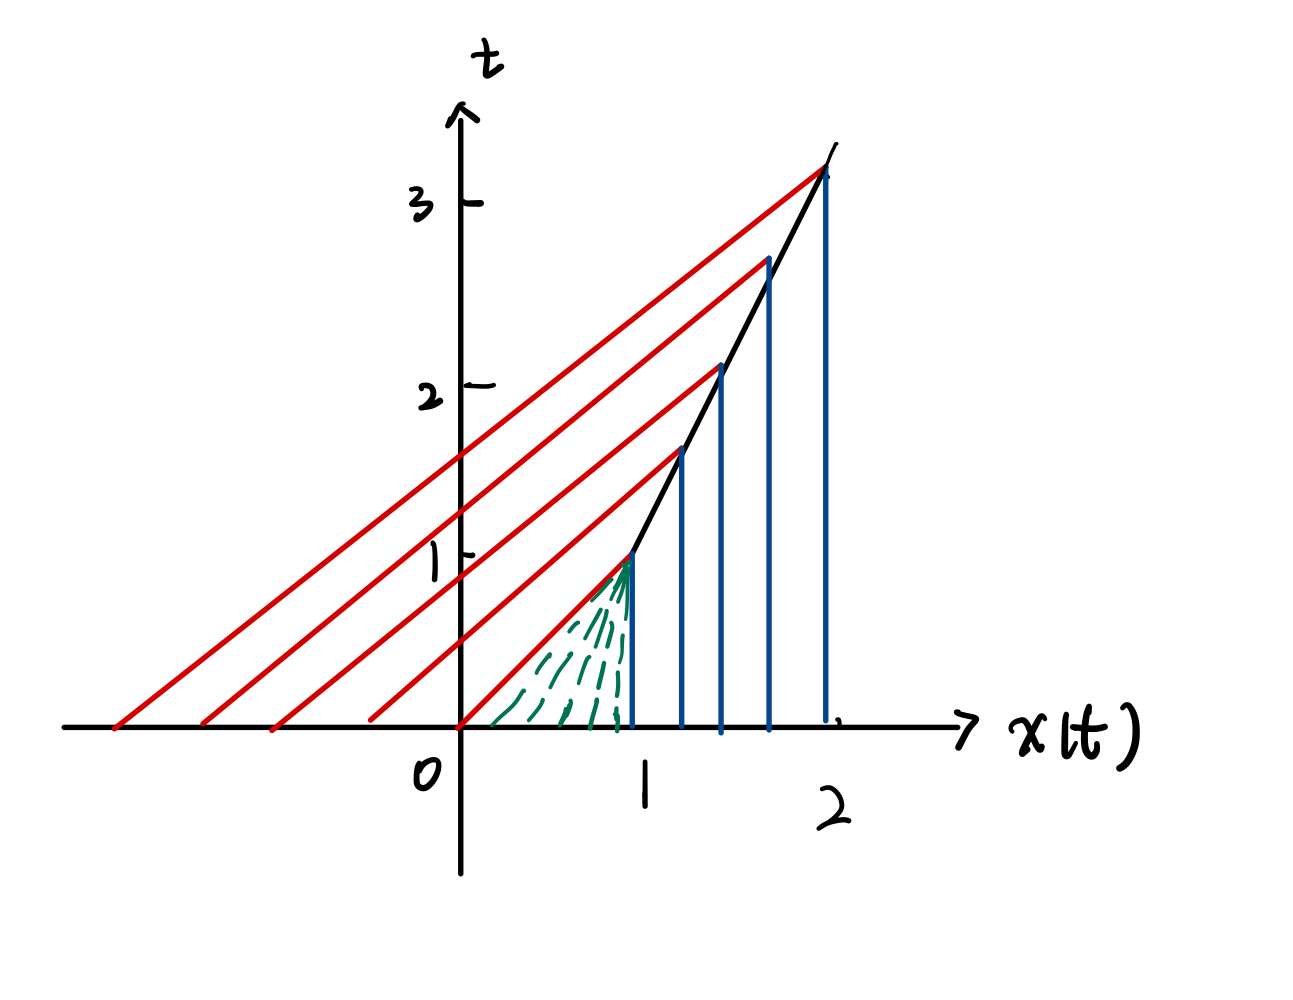
\includegraphics[width=0.51\textwidth]{Graph 2.jpeg} % Replace "filename" with the actual name of your image file
    %\caption{The characteristic lines}
    \label{fig:The second graph of characteristic lines}
  \end{figure}

Since $u(x,t)=u(x,0)=u(x_{0})$, the solution is 
\begin{equation*}u(x,t)=
    \begin{cases}
        1 & \text{ for } x \le t, x\le s(t+1),\\
        \frac{1-x}{1-t} & \text{ for } 0\le x\le 1\text{ and } x\ge t,\\
        0 & \text{ for }  x\ge 1 \text{ and } x\ge s(1+t).
    \end{cases}
\end{equation*}
%And for $1\le  x\le t$, there are three possible values, the characteristic lines may intersect each other. 


\iffalse
\begin{equation*}u(x,t)=
    \begin{cases}
        1 & \text{ for } x \le t\\
        \frac{1-x}{1-t} & \text{ for } t \le x \le 1  \text{ or } 1 \le x \le t \\
        0 & \text{ for }  x\ge 1 \text{ and } x\le 1
    \end{cases}
\end{equation*}
\fi



\end{document}